\section{Evaluation} \label{sec-eval}

We deployed and evaluated $NO^2$ on both a local high end cluster and the cloud. Two
representative applications, cap3 and ImageMagick, are chosen for being tested. We focus on
reducting the completion time of jobs. Besides, the overheads and computing resource usage of $NO^2$ are also measured.

The first application, Cap3, is a well known sequence assembly program in bioinformatics. 
There are many Expressed Sequence Tag (EST) sequence files in
FASTA format. So the job is split naturally according to the FASTA files. With the job
description engine and the shell script templates we provide, it is
simple to describe a job. The second application, ImageMagick, is a classic open
source picture processing tool. Gaussian blur is a filter of ImageMagick, and it blurs an
image by a Gaussian function to reduce image noise. This effect is widely used in graphics
software, also known as Gaussian smoothing. In this case, the job is rendering an image of
a huge size with Gaussian blur. The image is cut into small pieces with ImageMagick and
then is filtered. All pieces are joined together in the end.

We use two metrics for evaluation: job completion time and computing resource usage. As a
job consists of lots of tasks that are processed in parallel, we define the job completion time
as the duration between the submission of the job and the finish of all tasks.
\footnote{ There are several iterations in a workflow for most of the scientific computing jobs, 
 and the successor jobs depend on the precursor ones. For instance, the
precursor's output may be the the successor's input.} We run a job repeatedly
and use the average job completion time as the system metric. Considering
speculative executions call for extra computing resource, we also measure the computing
resource usage with CPU utilization, monitored by the ProActive Resource Manager. Given
the baseline and $NO^2$ CPU utilization, the cost of speculative executions can be
demonstrated.

$NO^2$ acts as an extension to the ProActive Scheduler. ProActive Scheduler is a high
level job scheduling system based on ProActive library. With ProActive Resource Manager,
jobs can be submitted and scheduled to use variable types of computing resources. A job is
described with a XML description.

\subsubsection{Outliers}
In a high end cluster, each server node has powerful CPU, sufficient memory, and is equipped
with the high performance network (e.g., InfiniBand) and usually a parallel file system. The heterogeneity
of hardware is limited. Will outliers come out in a short several-minute execution?

We randomly select a hundred JVM nodes, and submit a job with hundreds
of parallel tasks. The test is repeated in different periods of
day. We found that even in a several-minute execution, sometimes
there are a few outliers, and they appear on random server nodes and at different times.

\begin{figure}
\centering
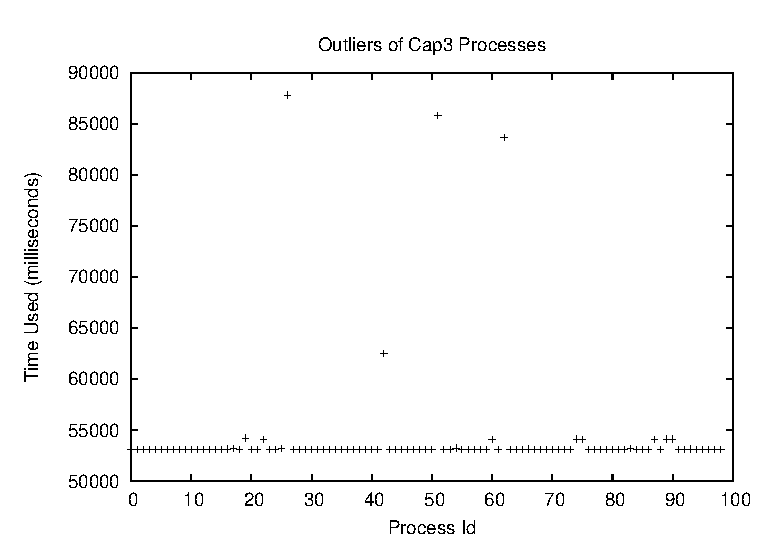
\includegraphics[width=0.9\columnwidth]{figures/outliers.eps}
\caption{Process durations of an Cap3 execution on 100 CPU cores in cluster at 8:00 am}
\label{figure:outlier}
\end{figure}

\begin{figure}
\centering
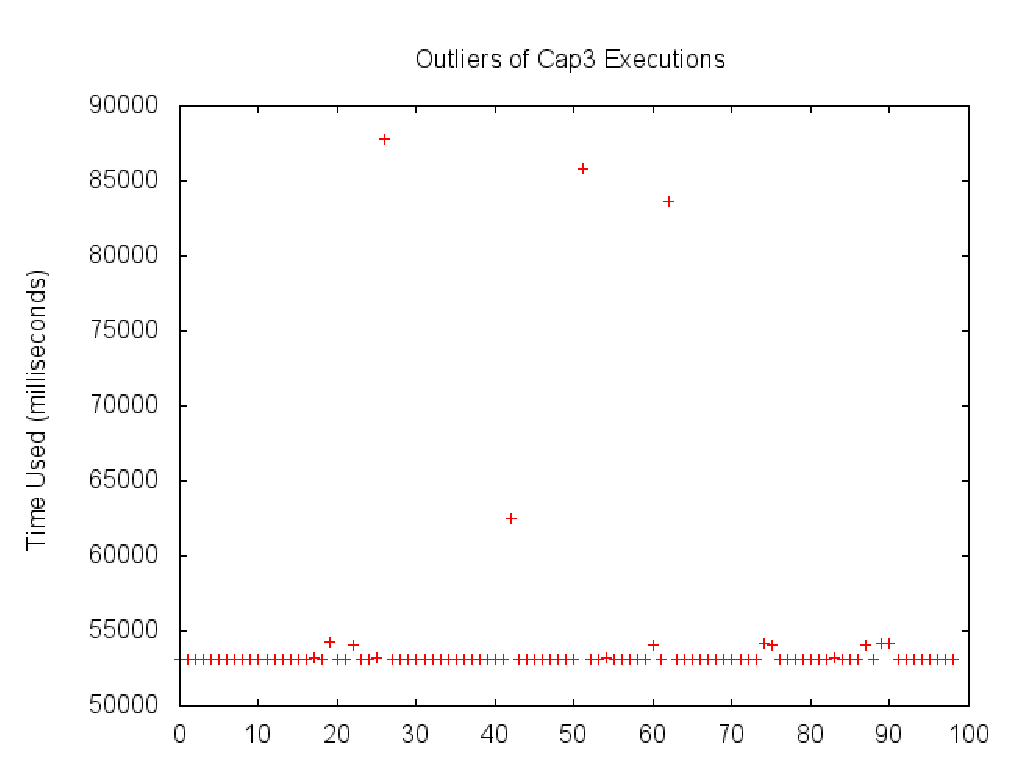
\includegraphics[width=0.9\columnwidth]{figures/yaoutliers.eps}
\caption{Process durations of an Cap3 execution on 100 CPU cores in cluster at 8:00 pm}
\label{figure:yaoutlier}
\end{figure}

We pick up two trials in this experiment, and make two scatter plots respectively as Fig.
\ref{figure:outlier} and Fig. \ref{figure:yaoutlier}. As shown in Fig.
\ref{figure:yaoutlier}, there are many more outliers than Fig. \ref{figure:outlier}, and
outliers need nearly twice the time to complete the same task. As one server node contains
several CPU cores, the physical outliers are not as many as outliers of CPU cores. With
this simple observation, we can conclude that even in high end clusters, there are a certain
number of outliers in some server nodes and during some periods of day, due to common computing resource
contention. For a further understanding about the outliers in the local cluster,
we loop this experiment several times to last a whole day. Fig.
\ref{figure:outlier_stats} has shown a rough statistics for the probability of outlier
each hour in one day.

\begin{figure}
\centering
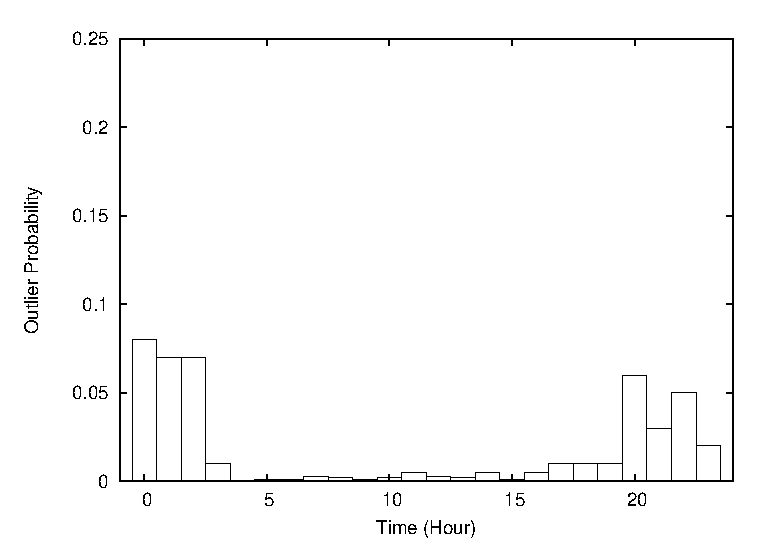
\includegraphics[width=0.9\columnwidth]{figures/outlier_stats.eps}
\caption{Probability of outliers during each hour of the day}
\label{figure:outlier_stats}
\end{figure}

As this experiment may produce some computing resource contentions and the data is just in
one day, the statistics is not accurate. For a non-quantitative study with the outliers, we
simply make an assumption that a CPU core of the cluster happens to be an outlier is a
random event, and the events are independent. As jobs often need lots of CPU cores to run
massive parallel tasks, the probability $P$ of a job running $N$ parallel tasks without
outlier is:

$$P = \prod_{i=1}^N p_i(t)$$

While $p_i(t)$ is the probability of $i$th task of the job happens \emph{not} to be a
outlier at time $t$, $\overline{p}_i(t)$ is the probability of $i$th task of the job
happens to be a outlier at time $t$. We choose the median of the Probability of outliers
shown in the Fig. \ref{figure:outlier_stats} $\overline{p}_i(17) = 0.01$, for a job having
100 parallel tasks, the probability of running without outliers $P$ is about 0.3660. When
the job scales up to 1000 parallel tasks, even with a very little probability of outlier
$\overline{p}_i(16) = 0.005$, the probability of running without outliers $P$ is about
0.0067, which means it is nearly impossible to keep away from outliers. So an
outlier-aware tasks scheduling is extremely needed for a job with massive parallel tasks.

\subsubsection{Overhead and Accuracy of Instrumentation}

Binary instrumentation often costs a very high overhead, which may be tens of times slower
than no instrumentation executions. Although the static binary instrumentation is more
efficient than the dynamic, usually tens of percent points of overhead is needed if
all function entries are traced, as shown in the Fig. \ref{figure:overhead_cap3} and
Fig. \ref{figure:overhead_gaussianblur}. Such high overhead prevents it from being used in production clusters.

To evaluate our progress trace approach, we run the cap3 and gaussianblur from ImageMagick
in one server node of the cluster. Each application is tested repeatedly with different
inputs. Fig. \ref{figure:overhead_cap3} and Fig. \ref{figure:overhead_gaussianblur} shows
the results of this experiment. On average, instrumentation with all function entries
costs 8\% - 11\% extra time to complete the execution, while instrumentation based on
function hits statistics in $NO^2$ needs only 0.03\% - 0.1\% extra time costs.

\begin{figure}
\centering
  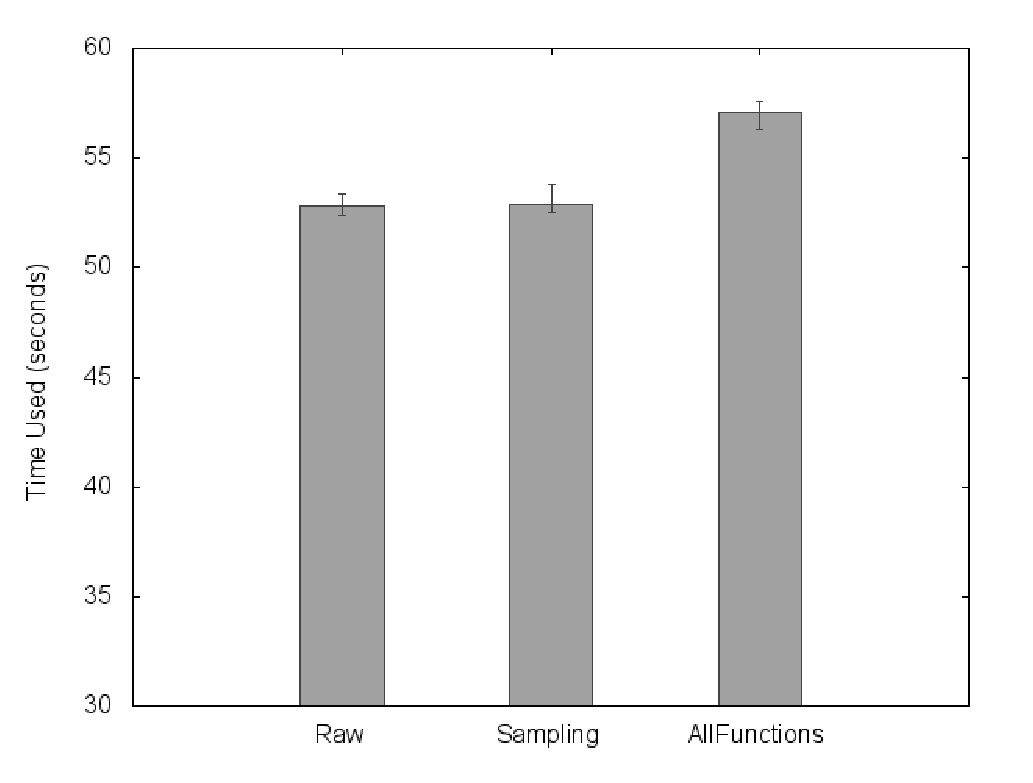
\includegraphics[width=0.9\columnwidth]{figures/overhead_cap3.eps}
\caption{Cap3 instrumentation overhead}
\label{figure:overhead_cap3}
\end{figure}

\begin{figure}
\centering
  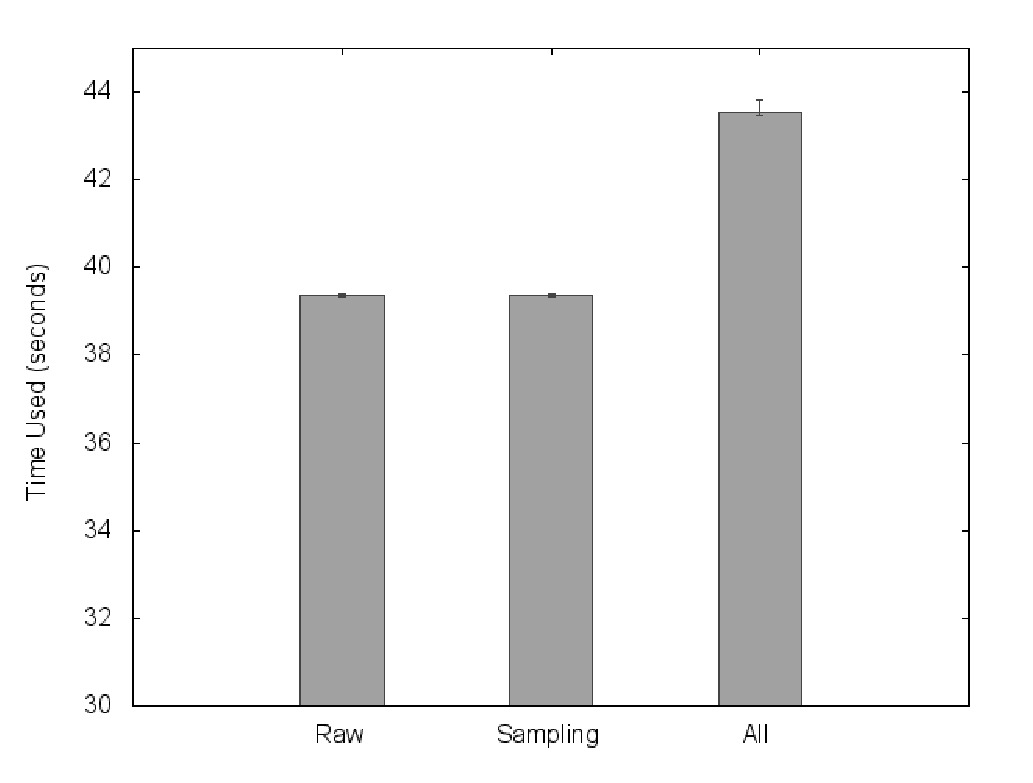
\includegraphics[width=0.9\columnwidth]{figures/overhead_gaussianblur.eps}
\caption{Gaussianblur instrumentation overhead}
\label{figure:overhead_gaussianblur}
\end{figure}

Such low overhead make $NO^2$ efficient enough to deploy on a production system. But
the tracpoints are uneven, which means the instrumentation may sometimes miss parts of progress and
the processes have caused progress to report inaccurate. So we make an inspection
with some trace cases of processes of Cap3, Gaussianblur and a combined image rendering
all from ImageMagick. We noticed that the progress trace with instrumentations with all
function entries is a little smoother than those with our instrumentation approach, such
as ImageMagick cases shows in Fig. \ref{figure:tracepoints}. But in some cases our
approach is a little smoother than instrumentation with all functions, such as Cap3 case
shows in Fig. \ref{figure:tracepoints}.

\begin{figure}
\centering
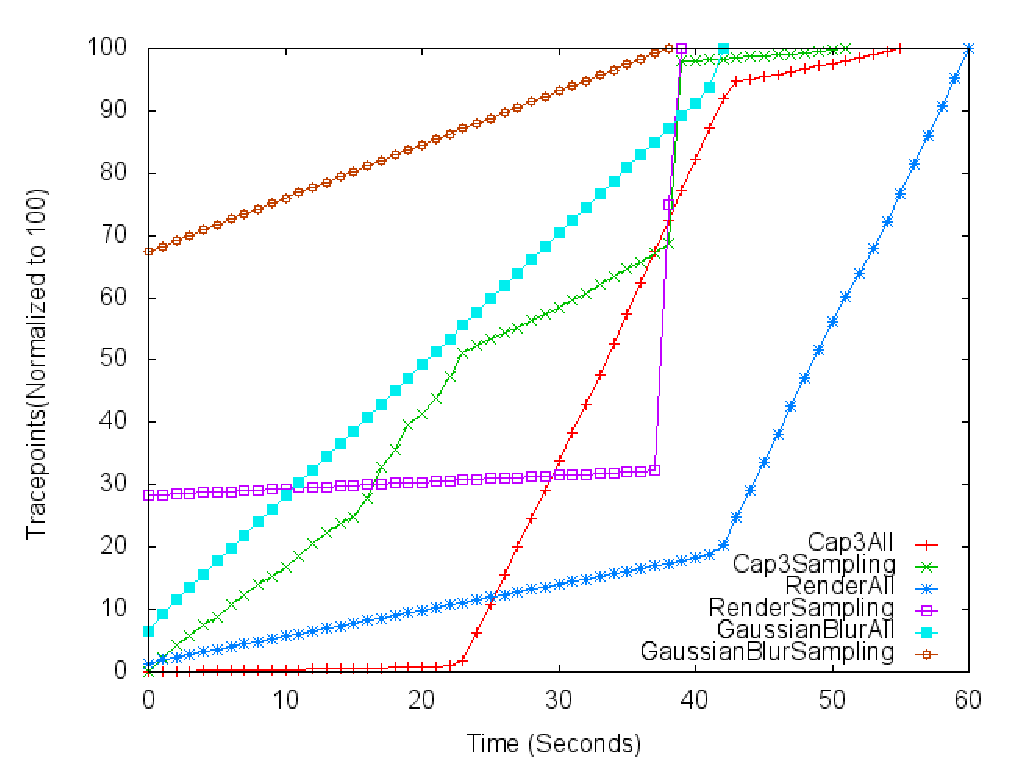
\includegraphics[width=0.9\columnwidth]{figures/tracepoints_all_vs_sampling.eps}
\caption{Skewed tracepoint accumulation over time}
\label{figure:tracepoints}
\end{figure}

Since each execution is completely arbitrary with different inputs and conditions, every
function may last short or long period of time in different executions. Unfortunately, we can
not make an inference of absolute execution progress with traces of instrumentation all
function entries. Even instrumentation with all basic binary blocks, there is no absolute
accuracy. A reasonable approach may be a customized instrumentation in kernel level,
requiring a modified Operating System kernel, with a large mount of time cost which is
nearly impossible to production system.

But a relative smooth tracepoints hit rate can be guaranteed with instrumentation function
entire in same granularity, as shown in Fig. \ref{figure:tracepoints}, each line is
composed of few smooth segments. The outliers clustering approach we proposed is inspired
by this inspection. We use the relative progress to catch the outliers, so the approach
instrumentation based on function hits statistics is enough to us.

\subsection{In Local Cluster}

The local cluster we used is a production one in Tsinghua University, which has hundreds
of  server nodes. While each node has tens of GBs of RAM and two Intel Xeon X5670 2.93 GHz
CPUs, each CPU has 6 cores. InfiniBand network and LUSTRE parallel file system are
deployed in the cluster. With Load Sharing Facility (LSF) job scheduling system, Hundreds
of Java Virtual Machines (JVMs) are launched as a LSF job in the cluster. These JVMs are
added as compute nodes in ProActive Resource Manager. We used the cluster just in this
way, adding the cluster as a LSF node source to the ProActive Resource Manager.

Reduction in job completion time is a critical metric. We submitted Cap3 and Gaussian Blur
jobs fifty times each to ProActive Scheduler with and without $NO^2$. Fig.
\ref{figure:completiontime_cap3} and Fig. \ref{figure:completiontime_gaussianblur} show
that job completion time has been improved by roughly 25\% on average. The histogram plots
the best, the worst, and the average reduction of Cap3 jobs and Gaussian Blur jobs. In the worst case
of Cap3, there is a little increment of job completion with $NO^2$, caused by a worst
choose in speculative execution. On average, the reduction of job completion time with
$NO^2$ is significant. Without $NO^2$, caused by the hinder of outliers, the completion
time of jobs has a big deviation with the best case. However with $NO^2$, the completion
time of jobs is reduced to the best case. These two experiments show that $NO^2$
mitigates the outliers efficiently.

\begin{figure}
\centering
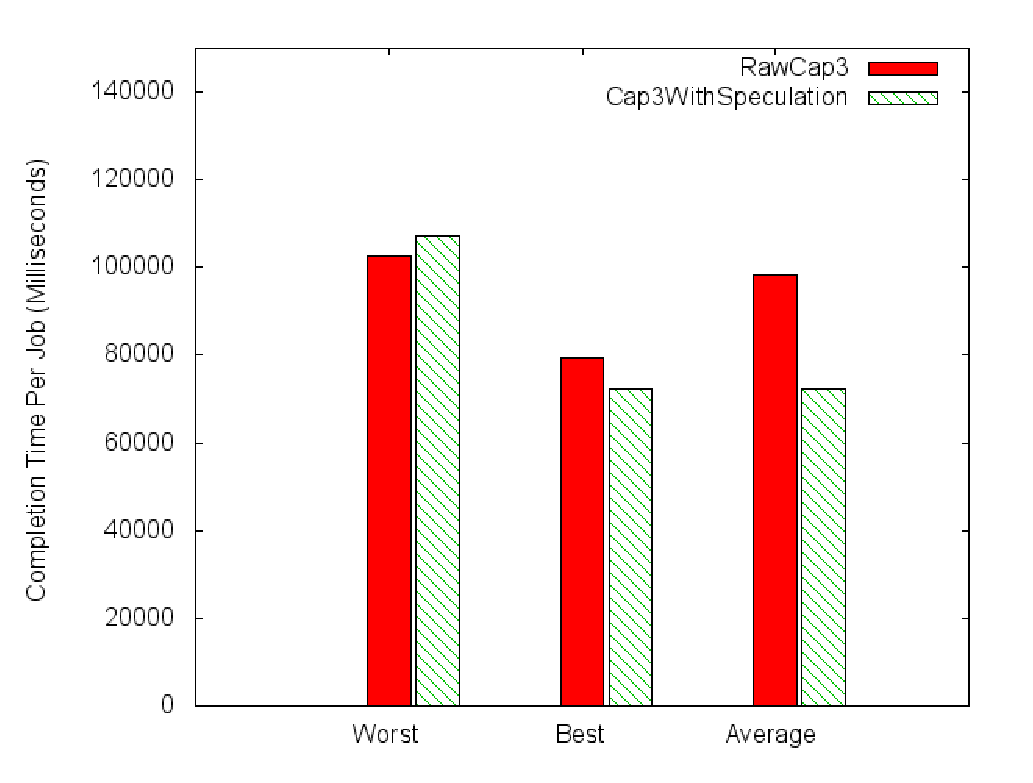
\includegraphics[width=0.9\columnwidth]{figures/completiontime_cap3.eps}
\caption{Completion time of Cap3 jobs}
\label{figure:completiontime_cap3}
\end{figure}

\begin{figure}
\centering
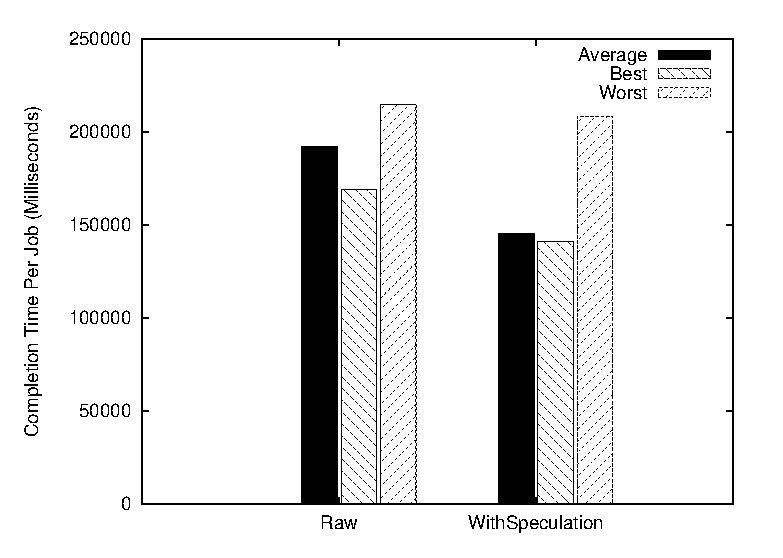
\includegraphics[width=0.9\columnwidth]{figures/completiontime_gaussianblur.eps}
\caption{Completion time of GaussianBlur jobs}
\label{figure:completiontime_gaussianblur}
\end{figure}

$NO^2$ can benefits job schedulers with reduction of job completion time. At
the same time, it needs some amount of computing resource in addition. In the aforementioned
test, we collected the statistics data of CPU usage from ProActive Resource Manager and
plotted a histogram as Fig. \ref{figure:resourceusage}.

\begin{figure}
\centering
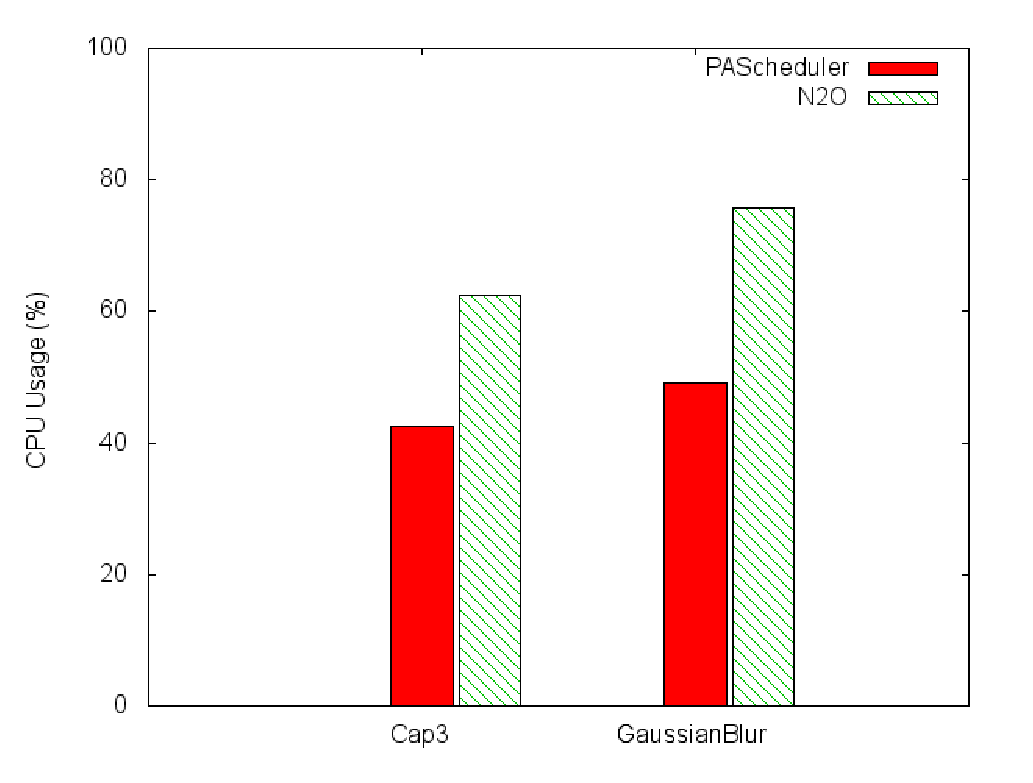
\includegraphics[width=0.9\columnwidth]{figures/resource_usage.eps}
\caption{Computing resource usage}
\label{figure:resourceusage}
\end{figure}

As shown in Fig. \ref{figure:resourceusage}, 20\% - 30\% more computing resource has been
used by $NO^2$ for speculative executions. This makes sense for some local clusters, which
has low utilization in most of the time of day. $NO^2$ helps them to scheduel jobs more
efficient, and reduces the server idle time. But for a busy cluster or cloud, where
computing resource is not free, we expect speculative executions use resource as little as
possible. We will analyze how to reduce waste of computing resource with little loss of
reduction of the job completion time later, and for some error-prone environment $NO^2$
can even use less computing resource with less failure executions.

\subsection{In Cloud}

With attractive low price and demand payment, there are more and more computing tasks
transferred to clouds in both academia and industry. The virtual clusters has been more
and more popular, StarCluster \cite{starcluster} is a toolkit for Amazon’s Elastic Compute
Cloud (EC2), designed to automate and simplify the process of building, configuring, and
managing clusters of virtual machines. We deployed such a virtual cluster on EC2 with
StarCluster. This cluster has hundreds of virtual machine nodes. Each node is a M1 small
instance, which has 1.7 GB RAM and one virtual CPU core with 1 EC2 Compute Unit. An
Elastic Block Storage (EBS) device is mounted as share storage and NFS file system is
deployed in the cluster. We deployed ProActive Scheduler on this virtual cluster like in
local cluster, with adding these virtual machine nodes as an SSHInfrastructure type node
source, Hundreds of Java Virtual Machines (JVMs) are launched and added as computing nodes
in ProActive Resource Manager.

We began our evaluation in the cloud by measuring the outliers, same as the verification
we have done in the local cluster. Unlike the high-end server nodes of local cluster, the
EC2 instances are mediocre and less powerful. The outliers in the cloud are more obvious
than the local cluster and prolong a 2X or more completion time for jobs, which has been
shown in Fig. \ref{figure:outlier_cloud}.

\begin{figure}
\centering
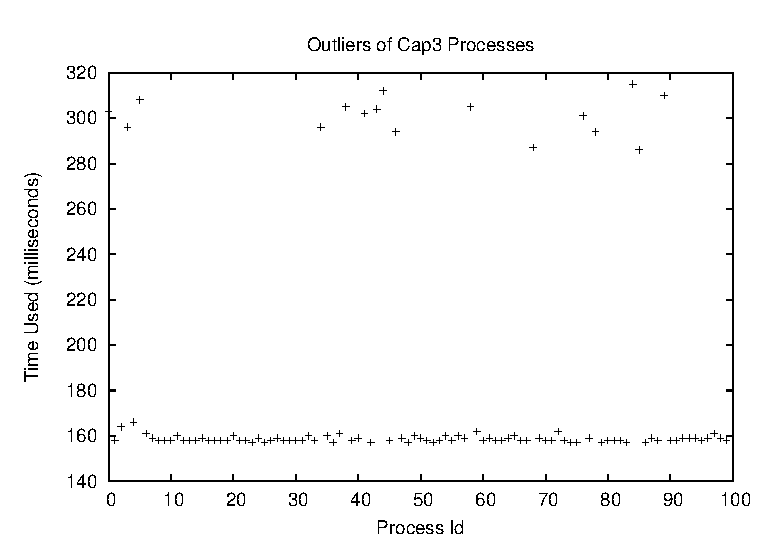
\includegraphics[width=0.9\columnwidth]{figures/cloud_outliers.eps}
\caption{Process durations of an Cap3 execution on 100 instances in cloud}
\label{figure:outlier_cloud}
\end{figure}

We submitted cap3 jobs in the same scale as local, and plot the histogram Fig.
\ref{figure:completiontime_cap3_cloud}. As computing resources is not sufficient in the
cloud, we also try an aborting strategy, also known as 'kill then restart' which costs less
computing resources than speculation. We will discuss this strategy in the next
section.

\begin{figure}
\centering
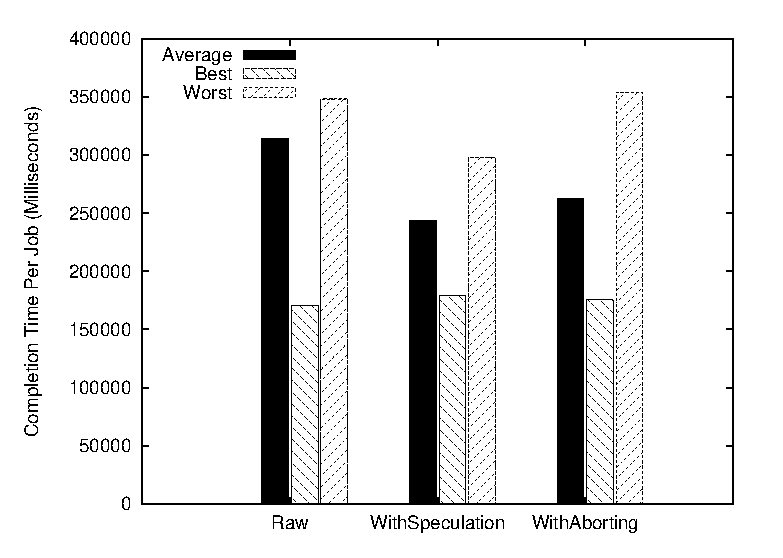
\includegraphics[width=0.9\columnwidth]{figures/cloud_completiontime_cap3.eps}
\caption{Completion time of Cap3 jobs in cloud}
\label{figure:completiontime_cap3_cloud}
\end{figure}

There is roughly 15\% - 22\% job completion time reduction on average shown in Fig.
\ref{figure:completiontime_cap3_cloud}. At the same time, the resource usage with
speculation strategy is 100\%, which means there may be more speculations not performed
for any sufficient computing resources and other jobs may be blocked with the same reason.
The aborting strategy is more economic, which only costs a 4\% - 5\% additional computing
resource.

\begin{figure}
\centering
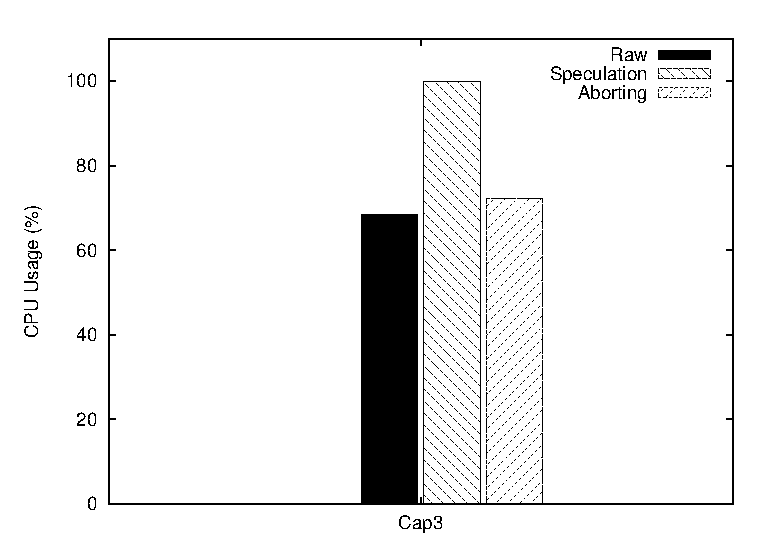
\includegraphics[width=0.9\columnwidth]{figures/cloud_resource_usage.eps}
\caption{Computing resource usage in cloud}
\label{figure:resourceusage_cloud}
\end{figure}

\section{Discussion} \label{sec-discussion}

We will make a discussion on the threshold tuning in $NO^2$ system in this section and take
one step further with $NO^2$ system by evaluation a different strategy to mitigate
outliers. These are two main pieces of experience we gain from varieties of practice.

\subsection{Threshold Tuning}

How slow will outliers mostly be? Or to what extent the process is lagged behind the majority when we could
judge it as an outlier? The threshold of outlier clusterings is critical for $NO^2$. In our
outlier clustering approach, we use a naive one-degree kmeans clustering algorithm where
$K = 2$, and we use the normalized variation of the centers of clusterings to judge if one
of them contains outliers. When the normalized variation is larger than a dynamic
threshold $T_d$, $NO^2$ realizes outliers exist. But the dynamic threshold $T_d$ depends
on the original threshold $T$ we determined a little arbitrarily. So a fine-grained tuning
with the threshold $T$ is an indispensable procedure for $NO^2$ system.

We use three fix JVM nodes running a shell script and costing lots of CPU to act as outliers.
In order to make sure other nodes are running normally, if there are some unexpected outliers, we
just drop the execution result. In this way, the other variation is limited. Tuning the
threshold $T$ from low to high, we run a Cap3 job which was split into 100 parallel tasks
to study the sensitivity of threshold $T$. In Fig. \ref{figure:thresholdtuning}, as
threshold rises, the number of waste speculations declines and keeps low, but successful
speculations have no obvious deviation. When threshold still increases, $NO^2$ finds out
little outliers and becomes lag to response.

\begin{figure}
\centering
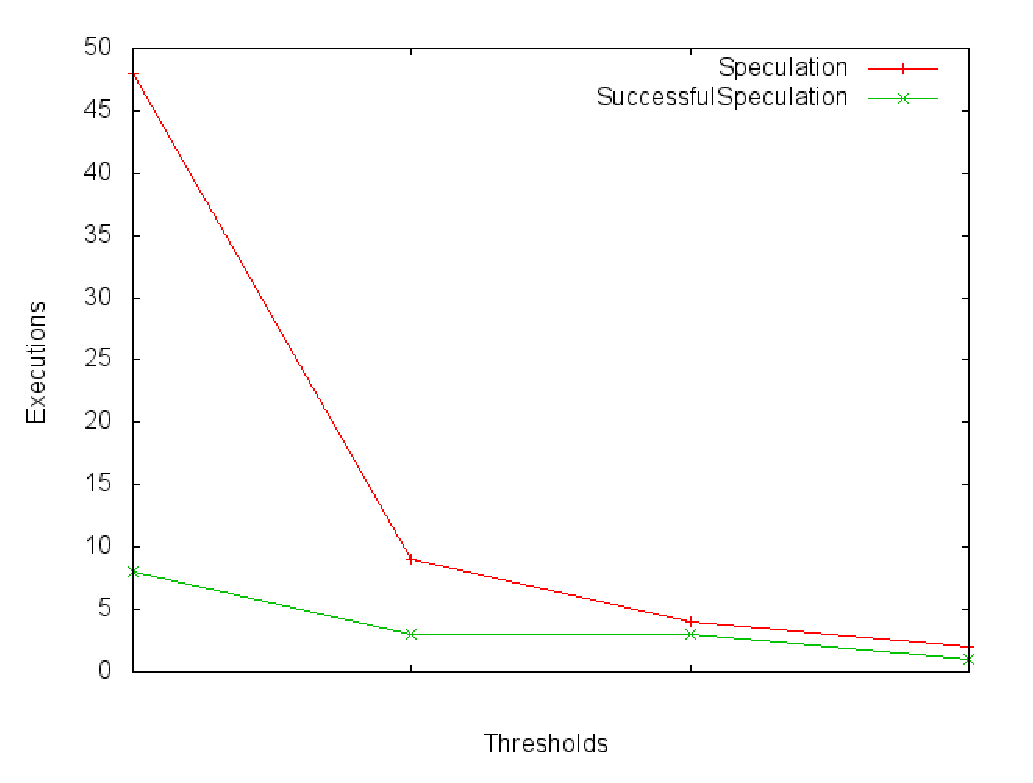
\includegraphics[width=0.9\columnwidth]{figures/threshold&speculation.eps}
\caption{Number of speculative executions over threshold values}
\label{figure:thresholdtuning}
\end{figure}

A low threshold may be false positive, and cause a large amount of speculative executions.
This has been shown in Fig.  \ref{figure:thresholdtuning}, which means a low success rate
of speculations and wastes a lot of computing resource. With an optimized threshold, our
outliers clustering approach can mitigate the false positive risks and keep sensitive with
outliers, this is critical for $NO^2$.

\subsection{Aborting Strategy}

Considering the idle computing resources may be not sufficient to meet the speculations'
need, such as in the cloud. We try an aborting strategy which is a bit different from
speculation. This strategy is more aggressive and adventurous. Rather than speculates, it
immediately aborts the potential outliers and restarts these tasks on another nodes not in
the blacklist. This extreme scheduling decision cuts lots of computing resources usage
which is needed for speculation, meanwhile may slow down the completion time of a job.
Because of that it is indeterminate if a speculative process will complete earlier than
the outlier.

We verified this strategy by repeating the same experiment with modified $NO^2$ system
equipmented with aborting scheduling strategy in the aforementioned local cluster. Fig.
\ref{figure:abort_completiontime_cap3} and Fig.
\ref{figure:abort_completiontime_gaussianblur} show that aborting strategy has a larger
variation than the speculation one in job completion time. In the worst case of Cap3 and
Gaussian Blur, aborting strategy is obviously slower than the case without $NO^2$ and with
$NO^2$'s speculation strategy. On average of Cap3 case, similar with
speculation strategy, aborting strategy reduces 25\% of job completion time. In contract, aborting
strategy has a slowdown in the Gaussian Blur case. There is nearly 10\% more time cost
than the speculation strategy. These two experiments show that aborting strategy can
reduce the completion time of jobs, but is a little slower than the speculation strategy.

\begin{figure}
\centering
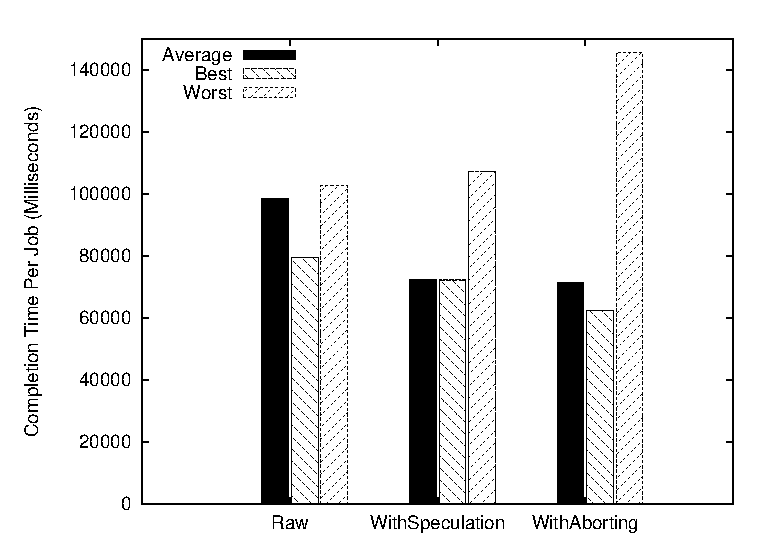
\includegraphics[width=0.9\columnwidth]{figures/abort_completiontime_cap3.eps}
\caption{Cap3 job completion time with aborting strategy}
\label{figure:abort_completiontime_cap3}
\end{figure}

\begin{figure}
\centering
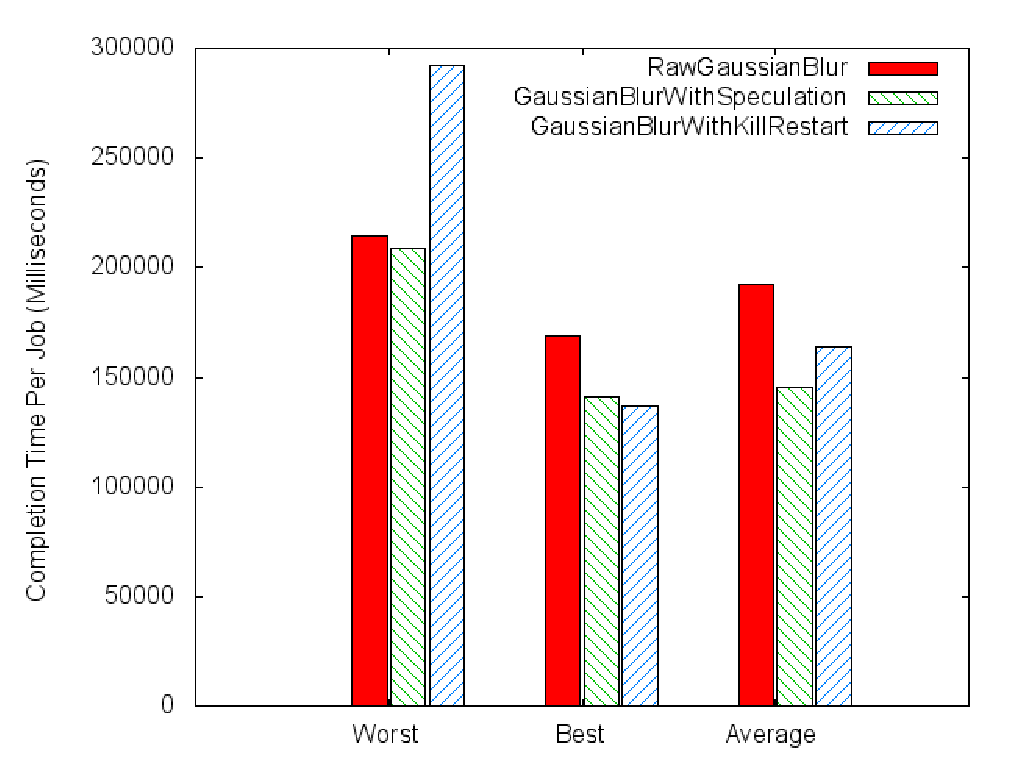
\includegraphics[width=0.9\columnwidth]{figures/abort_completiontime_gaussianblur.eps}
\caption{GaussianBlur job completion time with aborting strategy}
\label{figure:abort_completiontime_gaussianblur}
\end{figure}

With a little performance degraded, the aborting strategy cuts down lots of CPU resource
usage. The same as last experiment, we collected the statistics data of CPU usage from
ProActive Resource Manager and plotted a histogram as Fig.
\ref{figure:abort_resourceusage}.

\begin{figure}
\centering
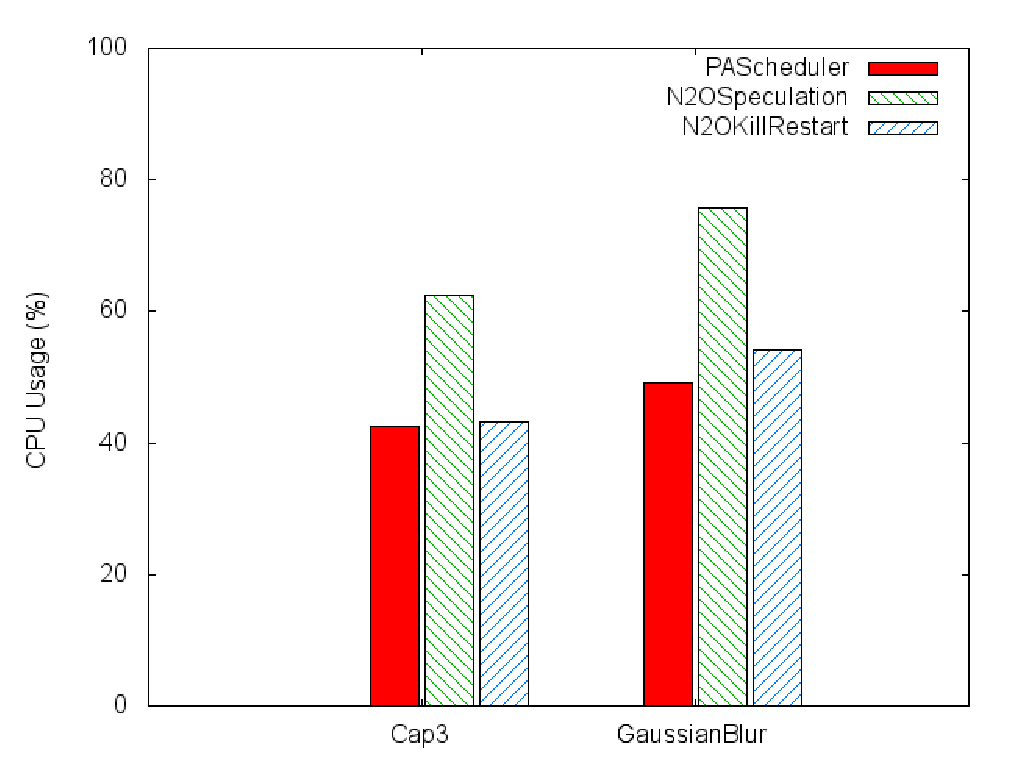
\includegraphics[width=0.9\columnwidth]{figures/abort_resource_usage.eps}
\caption{Computing resource usage of aborting strategy}
\label{figure:abort_resourceusage}
\end{figure}

As shown in Fig. \ref{figure:abort_resourceusage}, about 20\% CPU usage reduction
obtained. With the aborting strategy, the waste of CPU resource is bounded about 10\%,
which verified that the aborting strategy is valuable. This has also comfirmed by the
experiment in the cloud shown in Fig. \ref{figure:resourceusage_cloud}. 
